% !TeX root = ../mainfile.tex

\section{Basics}
Text can be \textbf{bold}, \textit{italic}, \underline{underlined} or \textbf{\textit{\underline{everything together}}}. \texttt{Inline code is possible too}. Another sentence.

Text indents automatically if you leaves one row empty. Lorem ipsum dolor sit amet, consetetur sadipscing elitr, sed diam nonumy eirmod tempor invidunt ut labore et dolore magna aliquyam erat, sed diam voluptua. At vero eos et accusam et justo duo dolores et ea rebum. Stet clita kasd gubergren, no sea takimata sanctus est Lorem ipsum dolor sit amet. Lorem ipsum dolor sit amet, consetetur sadipscing elitr, sed diam nonumy eirmod tempor invidunt ut labore et dolore magna aliquyam erat, sed diam voluptua. At vero eos et accusam et justo duo dolores et ea rebum. Stet clita kasd gubergren, no sea takimata sanctus est Lorem ipsum dolor sit amet. \cite{Albrecht2010}

Lorem ipsum dolor sit amet, consetetur sadipscing elitr, sed diam nonumy eirmod tempor invidunt ut labore et dolore magna aliquyam erat, sed diam voluptua. At vero eos et accusam et justo duo dolores et ea rebum. Stet clita kasd gubergren, no sea takimata sanctus est Lorem ipsum dolor sit amet. Lorem ipsum dolor sit amet, consetetur sadipscing elitr, sed diam nonumy eirmod tempor invidunt ut labore et dolore magna aliquyam erat, sed diam voluptua. At vero eos et accusam et justo duo dolores et ea rebum. Stet clita kasd gubergren, no sea takimata sanctus est Lorem ipsum dolor sit amet. \cite{hdl_routing} \cite{light_leakage_color}

\subsection{Item list}
\begin{itemize}
	\item item 1
	\subitem subitem 1
	\subitem subitem 2
	\item item 2
\end{itemize}

\subsection{Numbered List}
\begin{enumerate}
	\item numbered item 1
	\item numbered item 2
\end{enumerate}

\subsection{Table}
\begin{table}[H] %[] can be h (here), H (force here), ...
	\begin{center}
		\begin{tabular}{c|cc}
			& Item 1 & Item 2 \\
			\hline
			1 & c & d \\
			2 & e & f
		\end{tabular}
		\caption{Title.......}
		\label{tab:8bitnumber}
	\end{center}
\end{table}

\subsection{Math}
Inline Math looks like this $x = y + z$.
\begin{align}
	x &= y + z \\
	v + b &= 4
\end{align}

\begin{align*}
x &= y + z \\
v + b &= 4
\end{align*}

\pagebreak

\begin{figure}[H]
	\centering
	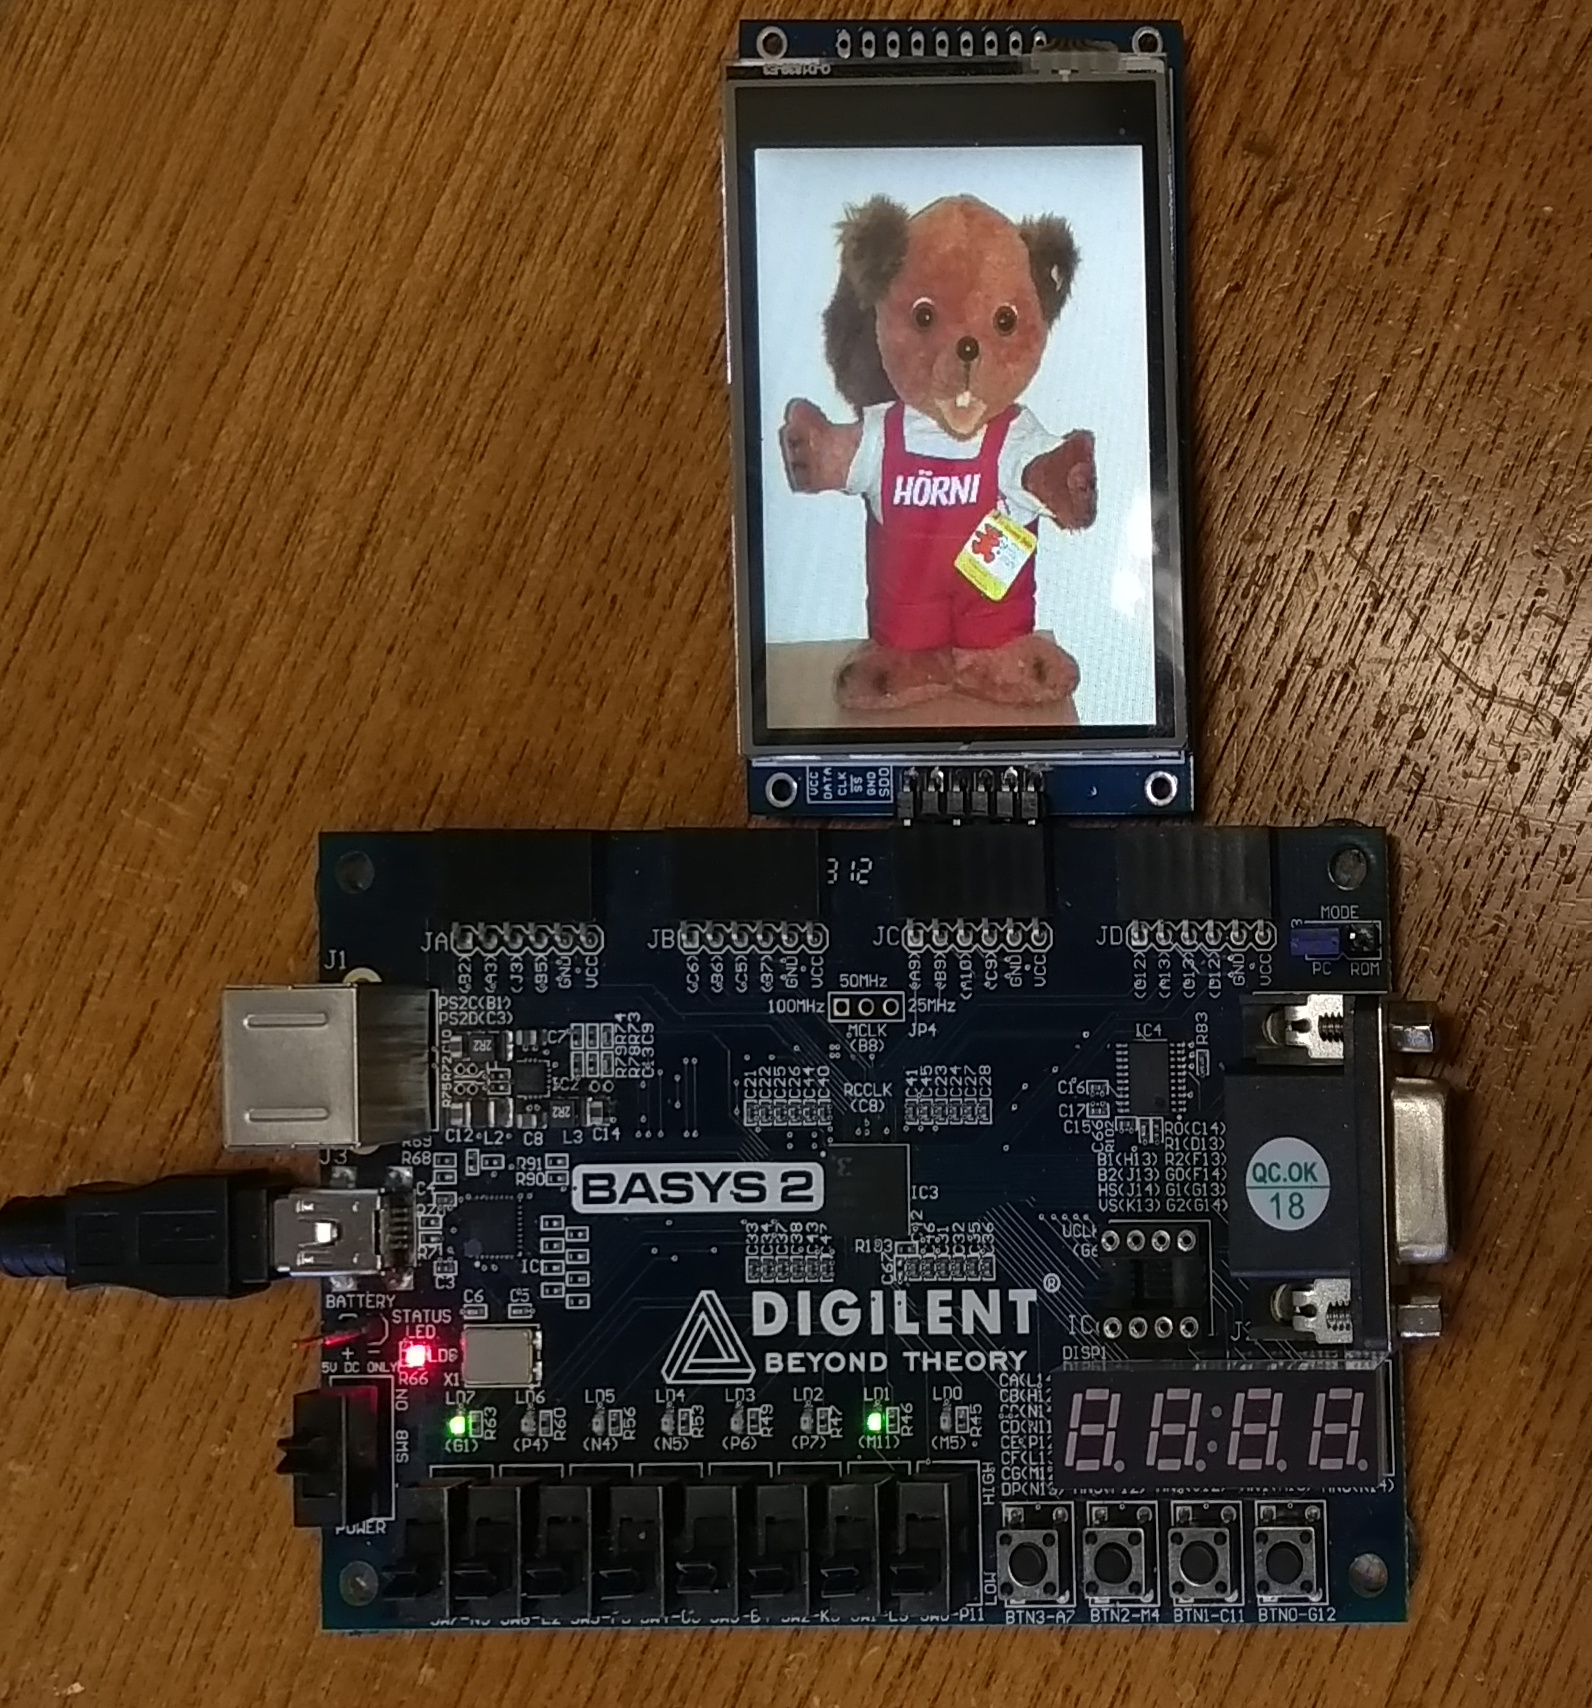
\includegraphics[width=0.5\linewidth]{inc/img/display_projekt/display_bsp_fpga}
	\caption{Basys 2 Board mit angeschlossenem Display an einem PMOD.}
	\label{fig:display_bespiel_angeschlossen}
\end{figure}

\pagebreak

\section{Layer 1}
asdf
\subsection{Layer 2}
asdf
\subsubsection{Layer 3}
asdf
\paragraph{Layer 4}
asdf
\subparagraph{Layer 5}
asdf